\documentclass[letterpaper,10pt,onecolumn]{article}
\usepackage[spanish]{babel}
\usepackage[latin1]{inputenc}
\usepackage{amsfonts}
\usepackage{amsthm}
\usepackage{amsmath}
\usepackage{mathrsfs}
\usepackage{empheq}
\usepackage{enumitem}
\usepackage[pdftex]{color,graphicx}
\usepackage{hyperref}
\usepackage{listings}
\usepackage{calligra}
\usepackage{algpseudocode} 
\DeclareMathAlphabet{\mathcalligra}{T1}{calligra}{m}{n}
\DeclareFontShape{T1}{calligra}{m}{n}{<->s*[2.2]callig15}{}
\newcommand{\scripty}[1]{\ensuremath{\mathcalligra{#1}}}
\lstloadlanguages{[5.2]Mathematica}
\setlength{\oddsidemargin}{0cm}
\setlength{\textwidth}{490pt}
\setlength{\topmargin}{-40pt}
\addtolength{\hoffset}{-0.3cm}
\addtolength{\textheight}{4cm}

\begin{document}
\begin{center}


\includegraphics[width=490pt]{header.png}\\[0.5cm]

\textsc{\LARGE Taller 2 - F\'isica I (FISI-1018) - 2015-10}\\[0.5cm]

\textsc{\Large{Profesor: Jaime Forero}} \\[0.5cm]

\noindent\textsc{Ejercicios correspondiente a la clase complementaria
  de la semana del 9 de Febrero del 2015.}\\[0.5cm]
\end{center}

\noindent\textsc{Nota:} Los primeros cuatro ejercicios deben ser
entregados {\bf al comienzo} de la clase complementaria. Los siguientes
cuatro deben ser trabajados durante la complementaria. Los cuatro {\bf
  ejercicios recomendados}  son para trabajo individual o consulta en
la Cl\'inica de Problemas. La numeraci\'on hace referencia al texto
gu\'ia: \textit{F\'isica Universitaria Volumen  1 (Sears-Semansky)},
decimotercera edici\'on, Pearson. 

\begin{enumerate}
\item Ejercicio 3.3 Dise\~nador de p\'aginas web.
\item Ejercicio 3.7 Trayectoria de un ave.
\item Ejercicio 3.10 Beisbolista de grandes ligas.
\item Ejercicio 3.24 Rotaci\'on de la Tierra.
\item Problema 3.71 Piedra en un acantilado.
\item Problema 3.49 Cuadrilla de demolici\'on.
\item Problema 3.56 Barco al frente del muelle.
\item Problema 3.60 Manguera para llenar un recipiente. 
\end{enumerate}

{\bf Ejercicios recomendados}\\
\begin{enumerate}
\item 
Encuentre el \'angulo entre los vectores $\vec{A}=3\hat{i}
-2\hat{j}+\hat{k}$ y $\vec{B}=-\hat{i}+3\hat{j}-2\hat{k}$.
\item Dos varillas largas forman un \'angulo $2\alpha$ entre
  ellas. Cada varilla se mueve perpendicularmente a s\'i misma con una
  rapidez $v$. �Cu\'al es la velocidad que tiene el punto de
  intersecci\'on de las varillas?
\item Una estudiante de F\'isica I se para en una colina y lanza una
  piedra formando un \'angulo $\theta$ con la horizontal. La pendiente
  de la colina baja con un \'angulo $\phi$. A que \'angulo $\theta$
  (que ser\'a una funci\'on de $\phi$) tiene que enviar la piedra para
  que recorra la m\'axima distancia posible sobre la colina? Ver
  diagrama de la Figura \ref{fig:tiro}.  
\item Una manera de medir la acelaraci\'on de la gravedad es lanzar
  alg\'un objeto hacia arriba y medir el tiempo que pasa en cruzar dos
  puntos diferentes en las dos direcciones. Muestre que si 
  $T_A$ es el tiempo que le toma al objeto pasar una l\'inea horizonal
  $A$ en ambas direcciones, y $T_B$ es el tiempo que le toma para pasar en dos
  direcciones por   otra l\'inea $B$, entonces la aceleraci\'on de la
  gravedad est\'a dada por:
  \begin{displaymath}
    g = \frac{8h}{T_A^2 -T_B^2}.
  \end{displaymath}
  Nota: ver la Figura \ref{fig:altura}. 
\end{enumerate}

\begin{figure}[!h]
\begin{center}
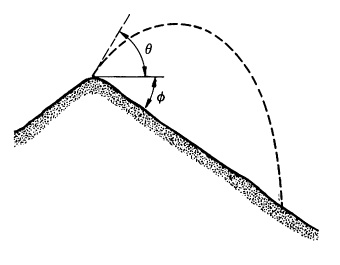
\includegraphics[scale=0.5]{figs/tiro.jpg} 
\end{center}
\caption{Diagrama para el ejercicio recomendado 3.}
\label{fig:tiro}
\end{figure}

\begin{figure}[!h]
\begin{center}
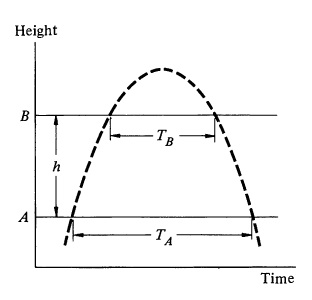
\includegraphics[scale=0.5]{figs/altura.jpg} 
\end{center}
\caption{Diagrama para el ejercicio recomendado 4.}
\label{fig:altura}
\end{figure}

\end{document}
